\subsection{Prima misura delle particelle alfa}
Sono stati settati gli strumenti, a pressione 600 $mb$.
Si è mantenuto lo Shaping Time a 0.25-0.5 $\mu s$, dopo aver osservato il comportamento. %dire cosa succede
E' stata regolata l'amplificazione in modo da mantenere il picco attorno ai $3V$.
E' stato impostato il trigger in modo tale che fosse circa a metà altezza del picco sull'oscilloscopio. 

%Avevamo visto che a 1,5 V dovevamo impostare circa 96 nel trigger in binario, ma poi, non ricordo per che motivo, abbiamo alzato a 128 tipo

Si è verificato che il numero di segnali spuri fosse inferiore al $30 \%$ del totale, facendo il grafico dei picchi e calcolando l'integrale dei segnali a bassa energia.

E' stato quindi acquisito il primo set di dati (circa 3000 eventi)

\begin{grafico}
 \centering
 \resizebox{\textwidth}{!}{%
 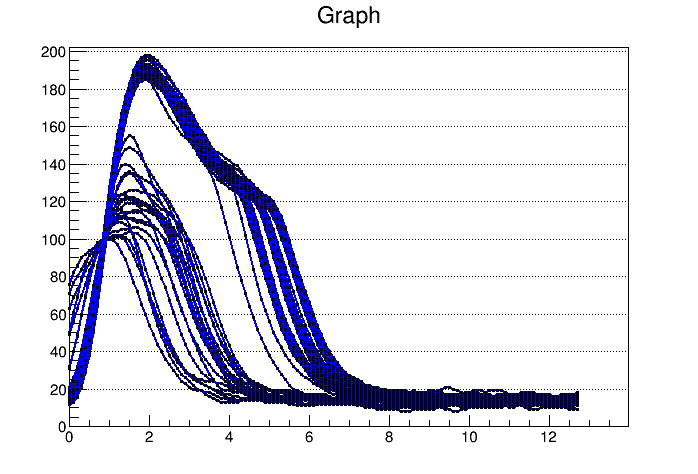
\includegraphics{../grafici/risultati/misura600.png}
 }%
 \caption{Grafico segnali a 600mb} 
 \label{gr:misura_600} 
\end{grafico}


E' stato acquisito anche un set di dati con meno eventi per stimare la baseline.
In particolare, è stato calcolato il centroide del picco della baseline, da inserire nella macro al posto del valore di default.

\begin{grafico}
 \centering
 \resizebox{\textwidth}{!}{%
 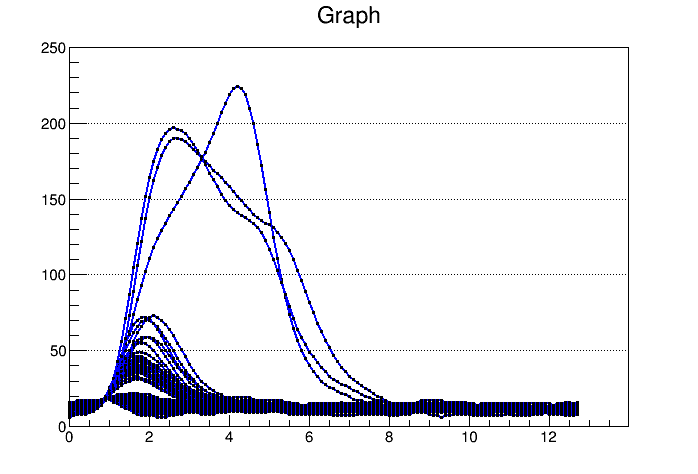
\includegraphics{../grafici/risultati/misura600fondo.png}
 }%
 \caption{Grafico segnali baseline} 
 \label{gr:misura600fondo} 
\end{grafico}

E' stato fatto il grafico degli integrali ed è stato calcolato il centroide del picco della baseline, da inserire nella macro al posto del valore di default.

\begin{grafico}
 \centering
 \resizebox{\textwidth}{!}{%
 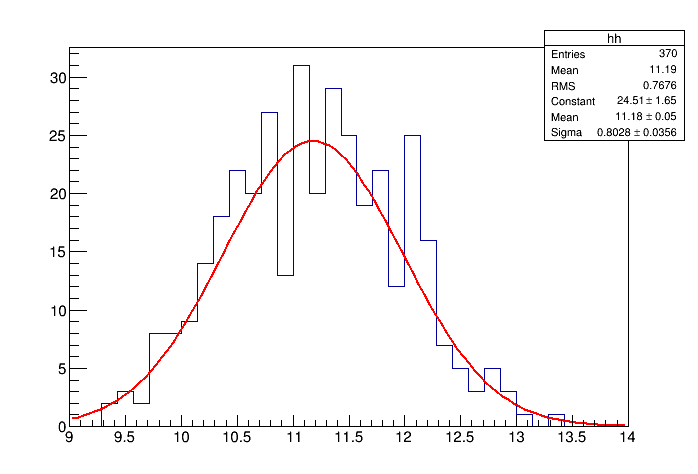
\includegraphics{../grafici/risultati/misura600fondo_baseline.png}
 }%
 \caption{Picco della baseline} 
 \label{gr:misura600fondo_baseline} 
\end{grafico}
%dati baseline

L'analisi dei dati che segue è stata effettuata utilizzando la macro fornite dal laboratorio,
modificando il limite dei campioni da integrare e inserendo il valore della baseline appena stimato.
Il limite dei campioni a 600 mb è stato posto uguale a 90.

\begin{grafico}
 \centering
 \resizebox{\textwidth}{!}{%
 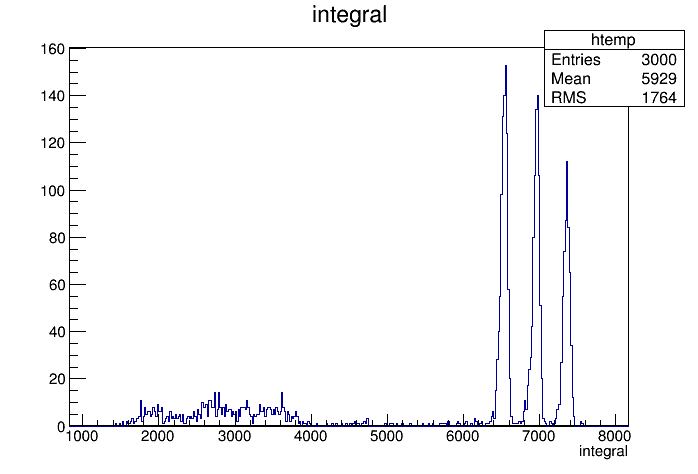
\includegraphics{../grafici/risultati/misura600_integral.png}
 }%
 \caption{Grafico integrale} 
 \label{gr:misura600_integral} 
\end{grafico}

 \begin{grafico}
 \centering
 \resizebox{\textwidth}{!}{%
 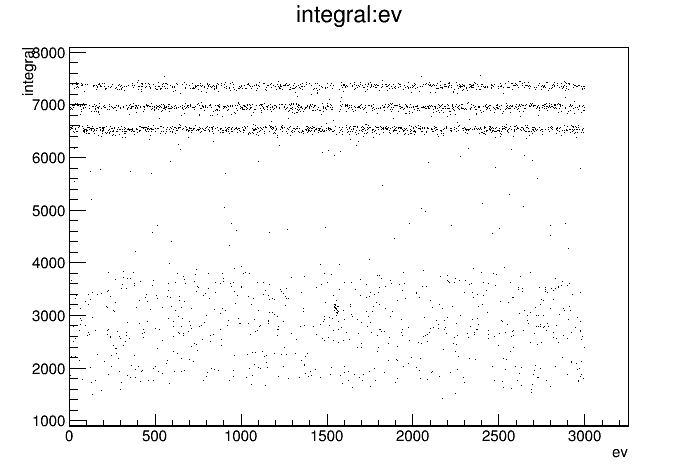
\includegraphics{../grafici/risultati/misura600_integral_ev.png}
 }%
 \caption{Grafico integral:ev} 
 \label{gr:misura600_integral_ev} 
\end{grafico}

 \begin{grafico}
 \centering
 \resizebox{\textwidth}{!}{%
 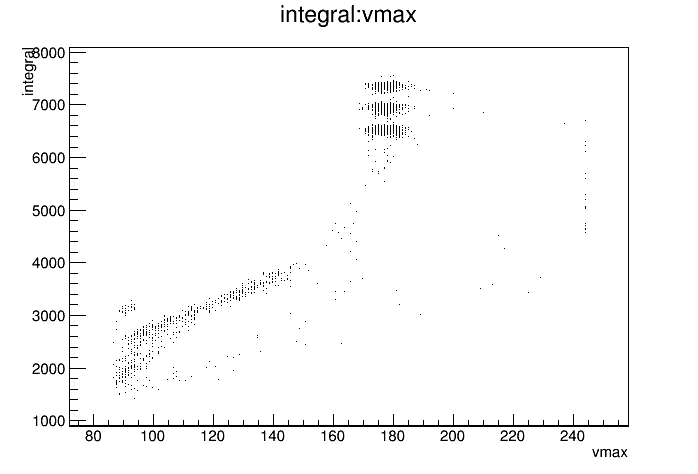
\includegraphics{../grafici/risultati/misura600_integral_vmax.png}
 }%
 \caption{Grafico integral:vmax} 
 \label{gr:misura600_integral_vmax} 
\end{grafico}

\begin{grafico}
 \centering
 \resizebox{\textwidth}{!}{%
 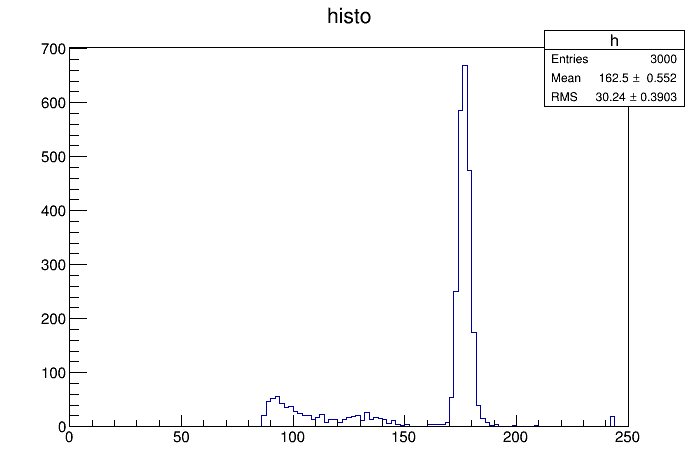
\includegraphics{../grafici/risultati/misura600_vmax.png}
 }%
 \caption{Grafico vmax} 
 \label{gr:misura600_vmax} 
\end{grafico}

 \begin{grafico}
 \centering
 \resizebox{\textwidth}{!}{%
 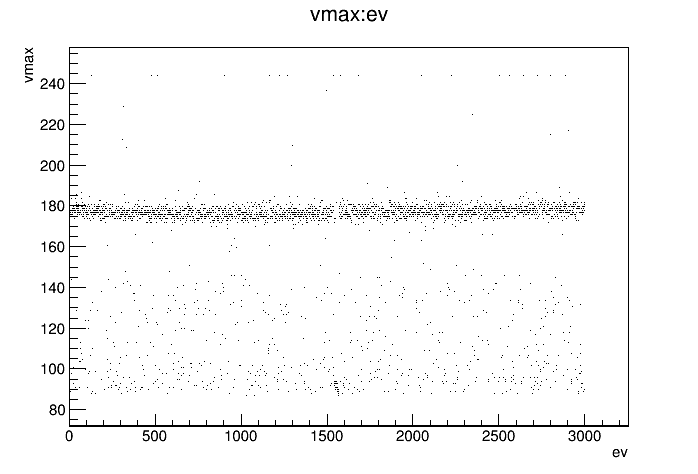
\includegraphics{../grafici/risultati/misura600_vmax_ev.png}
 }%
 \caption{Grafico vmax:ev} 
 \label{gr:misura600_vmax_ev} 
\end{grafico}

\subsection{Risoluzione energetica}
\subsection{Risoluzione energetica}
\FloatBarrier
Per il calcolo della risoluzione energetica, abbiamo per prima cosa trovata la relazione tra integrale ed energia, ipotizzandola lineare. 
Per fare ciò abbiamo calcolato l'energia teorica di ciscun picco, facendo la media delle energie dei decadimenti alfa, pesate sulla loro probabilità. 
Poi abbiamo calcolato l'integrale relativo a ciascun picco, come centroide del picco nell'istogramma degli integrali, e il suo errore, l'RMS del picco.
Da questi dati abbiamo proceduto ad un interpolazione dell'integrale in funzione dell'energia, ricavando così la funzione energia:integrale. 
Usando la funzione, abbiamo riscalato l'asse delle ascisse nell'istogramma degli integrali, in modo che mostrasse l'energia. 
Da questo nuovo istogramma abbiamo ricavato la risoluzione energetica, misurando l'RMS dei picchi e usandola per la formula

TODO fatemela bene voi la formula qui, non so fare le equazioni

$$risoluzione=\frac{2.335\cdot\sigma_E}{E}$$

\begin{grafico}
 \centering
 \resizebox{\textwidth}{!}{%
 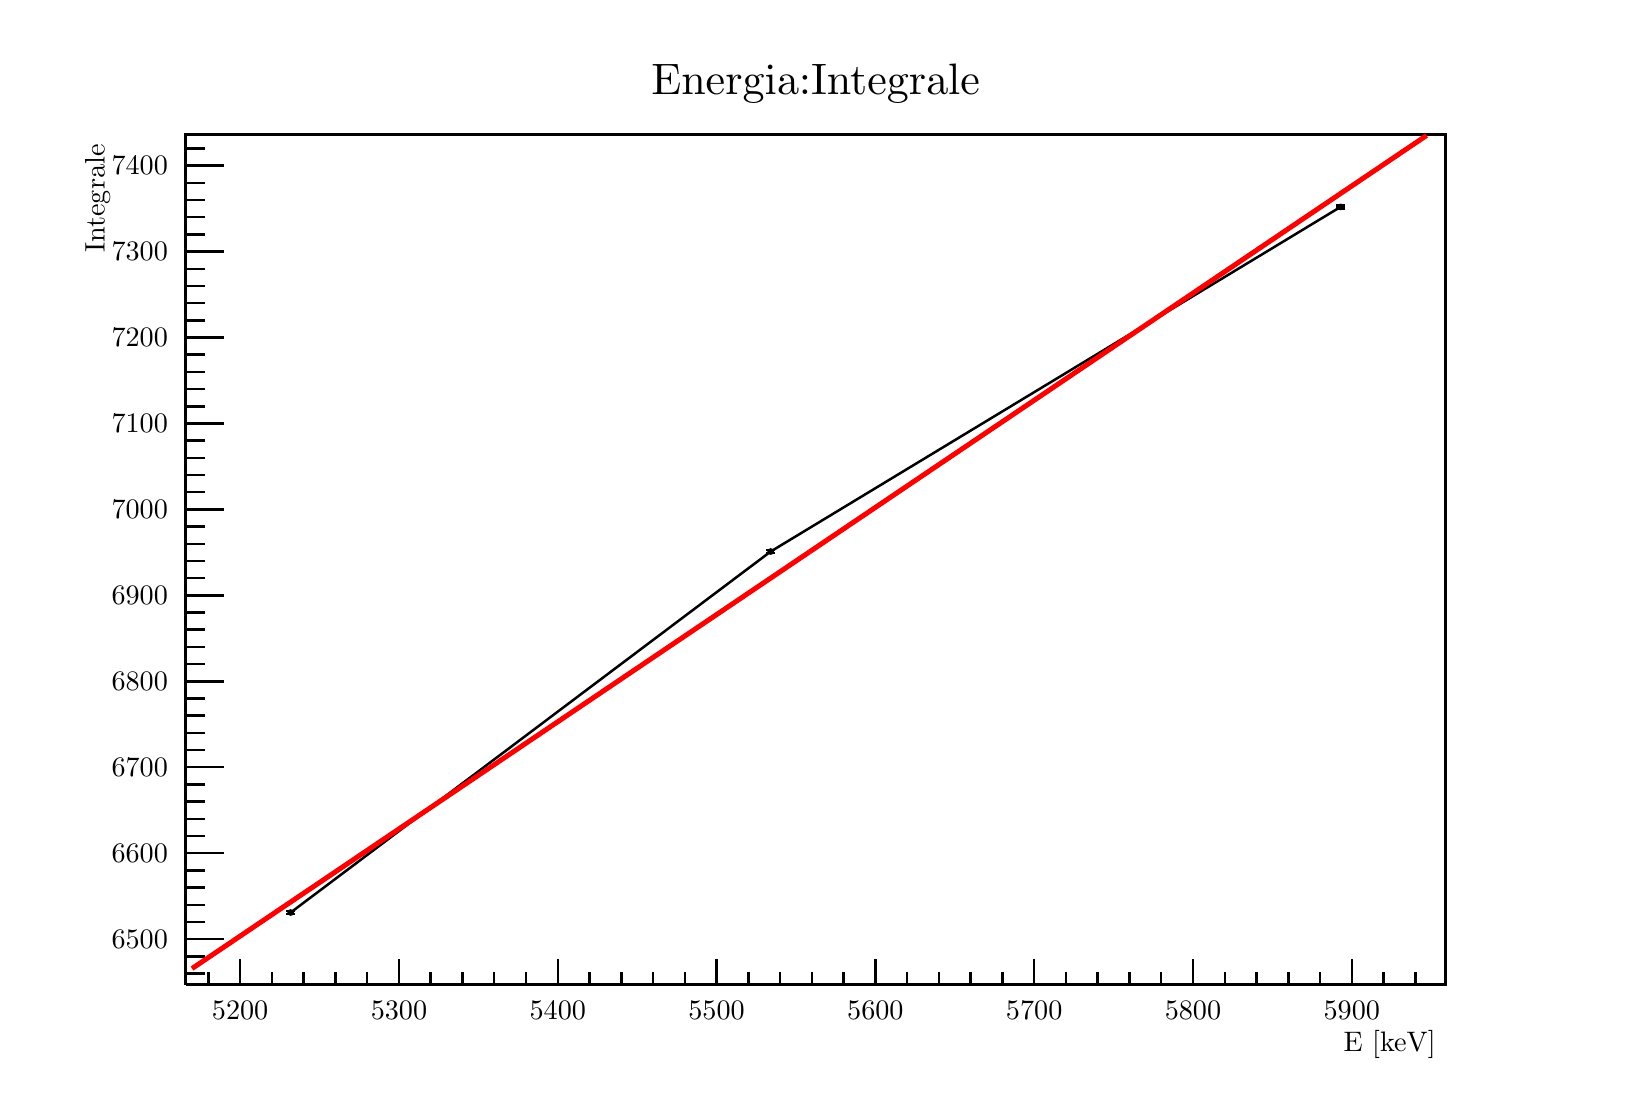
\begin{tikzpicture}
\pgfdeclareplotmark{cross} {
\pgfpathmoveto{\pgfpoint{-0.3\pgfplotmarksize}{\pgfplotmarksize}}
\pgfpathlineto{\pgfpoint{+0.3\pgfplotmarksize}{\pgfplotmarksize}}
\pgfpathlineto{\pgfpoint{+0.3\pgfplotmarksize}{0.3\pgfplotmarksize}}
\pgfpathlineto{\pgfpoint{+1\pgfplotmarksize}{0.3\pgfplotmarksize}}
\pgfpathlineto{\pgfpoint{+1\pgfplotmarksize}{-0.3\pgfplotmarksize}}
\pgfpathlineto{\pgfpoint{+0.3\pgfplotmarksize}{-0.3\pgfplotmarksize}}
\pgfpathlineto{\pgfpoint{+0.3\pgfplotmarksize}{-1.\pgfplotmarksize}}
\pgfpathlineto{\pgfpoint{-0.3\pgfplotmarksize}{-1.\pgfplotmarksize}}
\pgfpathlineto{\pgfpoint{-0.3\pgfplotmarksize}{-0.3\pgfplotmarksize}}
\pgfpathlineto{\pgfpoint{-1.\pgfplotmarksize}{-0.3\pgfplotmarksize}}
\pgfpathlineto{\pgfpoint{-1.\pgfplotmarksize}{0.3\pgfplotmarksize}}
\pgfpathlineto{\pgfpoint{-0.3\pgfplotmarksize}{0.3\pgfplotmarksize}}
\pgfpathclose
\pgfusepathqstroke
}
\pgfdeclareplotmark{cross*} {
\pgfpathmoveto{\pgfpoint{-0.3\pgfplotmarksize}{\pgfplotmarksize}}
\pgfpathlineto{\pgfpoint{+0.3\pgfplotmarksize}{\pgfplotmarksize}}
\pgfpathlineto{\pgfpoint{+0.3\pgfplotmarksize}{0.3\pgfplotmarksize}}
\pgfpathlineto{\pgfpoint{+1\pgfplotmarksize}{0.3\pgfplotmarksize}}
\pgfpathlineto{\pgfpoint{+1\pgfplotmarksize}{-0.3\pgfplotmarksize}}
\pgfpathlineto{\pgfpoint{+0.3\pgfplotmarksize}{-0.3\pgfplotmarksize}}
\pgfpathlineto{\pgfpoint{+0.3\pgfplotmarksize}{-1.\pgfplotmarksize}}
\pgfpathlineto{\pgfpoint{-0.3\pgfplotmarksize}{-1.\pgfplotmarksize}}
\pgfpathlineto{\pgfpoint{-0.3\pgfplotmarksize}{-0.3\pgfplotmarksize}}
\pgfpathlineto{\pgfpoint{-1.\pgfplotmarksize}{-0.3\pgfplotmarksize}}
\pgfpathlineto{\pgfpoint{-1.\pgfplotmarksize}{0.3\pgfplotmarksize}}
\pgfpathlineto{\pgfpoint{-0.3\pgfplotmarksize}{0.3\pgfplotmarksize}}
\pgfpathclose
\pgfusepathqfillstroke
}
\pgfdeclareplotmark{newstar} {
\pgfpathmoveto{\pgfqpoint{0pt}{\pgfplotmarksize}}
\pgfpathlineto{\pgfqpointpolar{44}{0.5\pgfplotmarksize}}
\pgfpathlineto{\pgfqpointpolar{18}{\pgfplotmarksize}}
\pgfpathlineto{\pgfqpointpolar{-20}{0.5\pgfplotmarksize}}
\pgfpathlineto{\pgfqpointpolar{-54}{\pgfplotmarksize}}
\pgfpathlineto{\pgfqpointpolar{-90}{0.5\pgfplotmarksize}}
\pgfpathlineto{\pgfqpointpolar{234}{\pgfplotmarksize}}
\pgfpathlineto{\pgfqpointpolar{198}{0.5\pgfplotmarksize}}
\pgfpathlineto{\pgfqpointpolar{162}{\pgfplotmarksize}}
\pgfpathlineto{\pgfqpointpolar{134}{0.5\pgfplotmarksize}}
\pgfpathclose
\pgfusepathqstroke
}
\pgfdeclareplotmark{newstar*} {
\pgfpathmoveto{\pgfqpoint{0pt}{\pgfplotmarksize}}
\pgfpathlineto{\pgfqpointpolar{44}{0.5\pgfplotmarksize}}
\pgfpathlineto{\pgfqpointpolar{18}{\pgfplotmarksize}}
\pgfpathlineto{\pgfqpointpolar{-20}{0.5\pgfplotmarksize}}
\pgfpathlineto{\pgfqpointpolar{-54}{\pgfplotmarksize}}
\pgfpathlineto{\pgfqpointpolar{-90}{0.5\pgfplotmarksize}}
\pgfpathlineto{\pgfqpointpolar{234}{\pgfplotmarksize}}
\pgfpathlineto{\pgfqpointpolar{198}{0.5\pgfplotmarksize}}
\pgfpathlineto{\pgfqpointpolar{162}{\pgfplotmarksize}}
\pgfpathlineto{\pgfqpointpolar{134}{0.5\pgfplotmarksize}}
\pgfpathclose
\pgfusepathqfillstroke
}
\definecolor{c}{rgb}{1,1,1};
\draw [color=c, fill=c] (0,0) rectangle (20,13.4957);
\draw [color=c, fill=c] (2,1.34957) rectangle (18,12.1461);
\definecolor{c}{rgb}{0,0,0};
\draw [c,line width=0.9] (2,1.34957) -- (2,12.1461) -- (18,12.1461) -- (18,1.34957) -- (2,1.34957);
\definecolor{c}{rgb}{1,1,1};
\draw [color=c, fill=c] (2,1.34957) rectangle (18,12.1461);
\definecolor{c}{rgb}{0,0,0};
\draw [c,line width=0.9] (2,1.34957) -- (2,12.1461) -- (18,12.1461) -- (18,1.34957) -- (2,1.34957);
\draw [c,line width=0.9] (2,1.34957) -- (18,1.34957);
\draw [anchor= east] (18,0.593811) node[scale=1.01821, color=c, rotate=0]{E [keV]};
\draw [c,line width=0.9] (2.6914,1.67347) -- (2.6914,1.34957);
\draw [c,line width=0.9] (3.09476,1.51152) -- (3.09476,1.34957);
\draw [c,line width=0.9] (3.49813,1.51152) -- (3.49813,1.34957);
\draw [c,line width=0.9] (3.90149,1.51152) -- (3.90149,1.34957);
\draw [c,line width=0.9] (4.30485,1.51152) -- (4.30485,1.34957);
\draw [c,line width=0.9] (4.70822,1.67347) -- (4.70822,1.34957);
\draw [c,line width=0.9] (5.11158,1.51152) -- (5.11158,1.34957);
\draw [c,line width=0.9] (5.51494,1.51152) -- (5.51494,1.34957);
\draw [c,line width=0.9] (5.9183,1.51152) -- (5.9183,1.34957);
\draw [c,line width=0.9] (6.32167,1.51152) -- (6.32167,1.34957);
\draw [c,line width=0.9] (6.72503,1.67347) -- (6.72503,1.34957);
\draw [c,line width=0.9] (7.12839,1.51152) -- (7.12839,1.34957);
\draw [c,line width=0.9] (7.53175,1.51152) -- (7.53175,1.34957);
\draw [c,line width=0.9] (7.93512,1.51152) -- (7.93512,1.34957);
\draw [c,line width=0.9] (8.33848,1.51152) -- (8.33848,1.34957);
\draw [c,line width=0.9] (8.74184,1.67347) -- (8.74184,1.34957);
\draw [c,line width=0.9] (9.1452,1.51152) -- (9.1452,1.34957);
\draw [c,line width=0.9] (9.54857,1.51152) -- (9.54857,1.34957);
\draw [c,line width=0.9] (9.95193,1.51152) -- (9.95193,1.34957);
\draw [c,line width=0.9] (10.3553,1.51152) -- (10.3553,1.34957);
\draw [c,line width=0.9] (10.7587,1.67347) -- (10.7587,1.34957);
\draw [c,line width=0.9] (11.162,1.51152) -- (11.162,1.34957);
\draw [c,line width=0.9] (11.5654,1.51152) -- (11.5654,1.34957);
\draw [c,line width=0.9] (11.9687,1.51152) -- (11.9687,1.34957);
\draw [c,line width=0.9] (12.3721,1.51152) -- (12.3721,1.34957);
\draw [c,line width=0.9] (12.7755,1.67347) -- (12.7755,1.34957);
\draw [c,line width=0.9] (13.1788,1.51152) -- (13.1788,1.34957);
\draw [c,line width=0.9] (13.5822,1.51152) -- (13.5822,1.34957);
\draw [c,line width=0.9] (13.9856,1.51152) -- (13.9856,1.34957);
\draw [c,line width=0.9] (14.3889,1.51152) -- (14.3889,1.34957);
\draw [c,line width=0.9] (14.7923,1.67347) -- (14.7923,1.34957);
\draw [c,line width=0.9] (15.1956,1.51152) -- (15.1956,1.34957);
\draw [c,line width=0.9] (15.599,1.51152) -- (15.599,1.34957);
\draw [c,line width=0.9] (16.0024,1.51152) -- (16.0024,1.34957);
\draw [c,line width=0.9] (16.4057,1.51152) -- (16.4057,1.34957);
\draw [c,line width=0.9] (16.8091,1.67347) -- (16.8091,1.34957);
\draw [c,line width=0.9] (2.6914,1.67347) -- (2.6914,1.34957);
\draw [c,line width=0.9] (2.28804,1.51152) -- (2.28804,1.34957);
\draw [c,line width=0.9] (16.8091,1.67347) -- (16.8091,1.34957);
\draw [c,line width=0.9] (17.2125,1.51152) -- (17.2125,1.34957);
\draw [c,line width=0.9] (17.6158,1.51152) -- (17.6158,1.34957);
\draw [anchor=base] (2.6914,0.904212) node[scale=1.01821, color=c, rotate=0]{5200};
\draw [anchor=base] (4.70822,0.904212) node[scale=1.01821, color=c, rotate=0]{5300};
\draw [anchor=base] (6.72503,0.904212) node[scale=1.01821, color=c, rotate=0]{5400};
\draw [anchor=base] (8.74184,0.904212) node[scale=1.01821, color=c, rotate=0]{5500};
\draw [anchor=base] (10.7587,0.904212) node[scale=1.01821, color=c, rotate=0]{5600};
\draw [anchor=base] (12.7755,0.904212) node[scale=1.01821, color=c, rotate=0]{5700};
\draw [anchor=base] (14.7923,0.904212) node[scale=1.01821, color=c, rotate=0]{5800};
\draw [anchor=base] (16.8091,0.904212) node[scale=1.01821, color=c, rotate=0]{5900};
\draw [c,line width=0.9] (2,1.34957) -- (2,12.1461);
\draw [anchor= east] (0.88,12.1461) node[scale=1.01821, color=c, rotate=90]{Integrale};
\draw [c,line width=0.9] (2.48,1.92711) -- (2,1.92711);
\draw [c,line width=0.9] (2.24,2.14541) -- (2,2.14541);
\draw [c,line width=0.9] (2.24,2.3637) -- (2,2.3637);
\draw [c,line width=0.9] (2.24,2.582) -- (2,2.582);
\draw [c,line width=0.9] (2.24,2.8003) -- (2,2.8003);
\draw [c,line width=0.9] (2.48,3.01859) -- (2,3.01859);
\draw [c,line width=0.9] (2.24,3.23689) -- (2,3.23689);
\draw [c,line width=0.9] (2.24,3.45518) -- (2,3.45518);
\draw [c,line width=0.9] (2.24,3.67348) -- (2,3.67348);
\draw [c,line width=0.9] (2.24,3.89178) -- (2,3.89178);
\draw [c,line width=0.9] (2.48,4.11007) -- (2,4.11007);
\draw [c,line width=0.9] (2.24,4.32837) -- (2,4.32837);
\draw [c,line width=0.9] (2.24,4.54666) -- (2,4.54666);
\draw [c,line width=0.9] (2.24,4.76496) -- (2,4.76496);
\draw [c,line width=0.9] (2.24,4.98326) -- (2,4.98326);
\draw [c,line width=0.9] (2.48,5.20155) -- (2,5.20155);
\draw [c,line width=0.9] (2.24,5.41985) -- (2,5.41985);
\draw [c,line width=0.9] (2.24,5.63814) -- (2,5.63814);
\draw [c,line width=0.9] (2.24,5.85644) -- (2,5.85644);
\draw [c,line width=0.9] (2.24,6.07474) -- (2,6.07474);
\draw [c,line width=0.9] (2.48,6.29303) -- (2,6.29303);
\draw [c,line width=0.9] (2.24,6.51133) -- (2,6.51133);
\draw [c,line width=0.9] (2.24,6.72962) -- (2,6.72962);
\draw [c,line width=0.9] (2.24,6.94792) -- (2,6.94792);
\draw [c,line width=0.9] (2.24,7.16621) -- (2,7.16621);
\draw [c,line width=0.9] (2.48,7.38451) -- (2,7.38451);
\draw [c,line width=0.9] (2.24,7.60281) -- (2,7.60281);
\draw [c,line width=0.9] (2.24,7.8211) -- (2,7.8211);
\draw [c,line width=0.9] (2.24,8.0394) -- (2,8.0394);
\draw [c,line width=0.9] (2.24,8.2577) -- (2,8.2577);
\draw [c,line width=0.9] (2.48,8.47599) -- (2,8.47599);
\draw [c,line width=0.9] (2.24,8.69429) -- (2,8.69429);
\draw [c,line width=0.9] (2.24,8.91258) -- (2,8.91258);
\draw [c,line width=0.9] (2.24,9.13088) -- (2,9.13088);
\draw [c,line width=0.9] (2.24,9.34917) -- (2,9.34917);
\draw [c,line width=0.9] (2.48,9.56747) -- (2,9.56747);
\draw [c,line width=0.9] (2.24,9.78577) -- (2,9.78577);
\draw [c,line width=0.9] (2.24,10.0041) -- (2,10.0041);
\draw [c,line width=0.9] (2.24,10.2224) -- (2,10.2224);
\draw [c,line width=0.9] (2.24,10.4407) -- (2,10.4407);
\draw [c,line width=0.9] (2.48,10.659) -- (2,10.659);
\draw [c,line width=0.9] (2.24,10.8772) -- (2,10.8772);
\draw [c,line width=0.9] (2.24,11.0955) -- (2,11.0955);
\draw [c,line width=0.9] (2.24,11.3138) -- (2,11.3138);
\draw [c,line width=0.9] (2.24,11.5321) -- (2,11.5321);
\draw [c,line width=0.9] (2.48,11.7504) -- (2,11.7504);
\draw [c,line width=0.9] (2.48,1.92711) -- (2,1.92711);
\draw [c,line width=0.9] (2.24,1.70882) -- (2,1.70882);
\draw [c,line width=0.9] (2.24,1.49052) -- (2,1.49052);
\draw [c,line width=0.9] (2.48,11.7504) -- (2,11.7504);
\draw [c,line width=0.9] (2.24,11.9687) -- (2,11.9687);
\draw [anchor= east] (1.9,1.92711) node[scale=1.01821, color=c, rotate=0]{6500};
\draw [anchor= east] (1.9,3.01859) node[scale=1.01821, color=c, rotate=0]{6600};
\draw [anchor= east] (1.9,4.11007) node[scale=1.01821, color=c, rotate=0]{6700};
\draw [anchor= east] (1.9,5.20155) node[scale=1.01821, color=c, rotate=0]{6800};
\draw [anchor= east] (1.9,6.29303) node[scale=1.01821, color=c, rotate=0]{6900};
\draw [anchor= east] (1.9,7.38451) node[scale=1.01821, color=c, rotate=0]{7000};
\draw [anchor= east] (1.9,8.47599) node[scale=1.01821, color=c, rotate=0]{7100};
\draw [anchor= east] (1.9,9.56747) node[scale=1.01821, color=c, rotate=0]{7200};
\draw [anchor= east] (1.9,10.659) node[scale=1.01821, color=c, rotate=0]{7300};
\draw [anchor= east] (1.9,11.7504) node[scale=1.01821, color=c, rotate=0]{7400};
\draw [c,line width=0.9] (3.33333,2.26547) -- (9.42909,6.84969) -- (16.6667,11.2265);
\foreach \P in {(3.33333,2.26547), (9.42909,6.84969), (16.6667,11.2265)}{\draw[mark options={color=c,fill=c},mark size=2.402402pt,mark=*,mark size=1pt] plot coordinates {\P};}
\definecolor{c}{rgb}{1,0,0};
\draw [c,line width=1.8] (2.08,1.55317) -- (2.24,1.66114) -- (2.4,1.76911) -- (2.56,1.87708) -- (2.72,1.98505) -- (2.88,2.09301) -- (3.04,2.20098) -- (3.2,2.30895) -- (3.36,2.41692) -- (3.52,2.52489) -- (3.68,2.63286) -- (3.84,2.74083) -- (4,2.8488)
 -- (4.16,2.95677) -- (4.32,3.06474) -- (4.48,3.17271) -- (4.64,3.28068) -- (4.8,3.38865) -- (4.96,3.49662) -- (5.12,3.60458) -- (5.28,3.71255) -- (5.44,3.82052) -- (5.6,3.92849) -- (5.76,4.03646) -- (5.92,4.14443) -- (6.08,4.2524) -- (6.24,4.36037)
 -- (6.4,4.46834) -- (6.56,4.57631) -- (6.72,4.68428) -- (6.88,4.79225) -- (7.04,4.90022) -- (7.2,5.00819) -- (7.36,5.11616) -- (7.52,5.22412) -- (7.68,5.33209) -- (7.84,5.44006) -- (8,5.54803) -- (8.16,5.656) -- (8.32,5.76397) -- (8.48,5.87194) --
 (8.64,5.97991) -- (8.8,6.08788) -- (8.96,6.19585) -- (9.12,6.30382) -- (9.28,6.41179) -- (9.44,6.51976) -- (9.6,6.62773) -- (9.76,6.7357) -- (9.92,6.84366);
\draw [c,line width=1.8] (9.92,6.84366) -- (10.08,6.95163) -- (10.24,7.0596) -- (10.4,7.16757) -- (10.56,7.27554) -- (10.72,7.38351) -- (10.88,7.49148) -- (11.04,7.59945) -- (11.2,7.70742) -- (11.36,7.81539) -- (11.52,7.92336) -- (11.68,8.03133) --
 (11.84,8.1393) -- (12,8.24727) -- (12.16,8.35524) -- (12.32,8.4632) -- (12.48,8.57117) -- (12.64,8.67914) -- (12.8,8.78711) -- (12.96,8.89508) -- (13.12,9.00305) -- (13.28,9.11102) -- (13.44,9.21899) -- (13.6,9.32696) -- (13.76,9.43493) --
 (13.92,9.5429) -- (14.08,9.65087) -- (14.24,9.75884) -- (14.4,9.86681) -- (14.56,9.97478) -- (14.72,10.0827) -- (14.88,10.1907) -- (15.04,10.2987) -- (15.2,10.4067) -- (15.36,10.5146) -- (15.52,10.6226) -- (15.68,10.7306) -- (15.84,10.8385) --
 (16,10.9465) -- (16.16,11.0545) -- (16.32,11.1624) -- (16.48,11.2704) -- (16.64,11.3784) -- (16.8,11.4863) -- (16.96,11.5943) -- (17.12,11.7023) -- (17.28,11.8103) -- (17.44,11.9182) -- (17.6,12.0262) -- (17.76,12.1342);
\definecolor{c}{rgb}{0,0,0};
\draw [c,line width=0.9] (3.33333,2.26547) -- (3.33333,2.28166);
\draw [c,line width=0.9] (3.27603,2.28166) -- (3.39064,2.28166);
\draw [c,line width=0.9] (3.33333,2.26547) -- (3.33333,2.24928);
\draw [c,line width=0.9] (3.27603,2.24928) -- (3.39064,2.24928);
\draw [c,line width=0.9] (9.42909,6.84969) -- (9.42909,6.86865);
\draw [c,line width=0.9] (9.37178,6.86865) -- (9.4864,6.86865);
\draw [c,line width=0.9] (9.42909,6.84969) -- (9.42909,6.83073);
\draw [c,line width=0.9] (9.37178,6.83073) -- (9.4864,6.83073);
\draw [c,line width=0.9] (16.6667,11.2265) -- (16.6667,11.2464);
\draw [c,line width=0.9] (16.6094,11.2464) -- (16.724,11.2464);
\draw [c,line width=0.9] (16.6667,11.2265) -- (16.6667,11.2066);
\draw [c,line width=0.9] (16.6094,11.2066) -- (16.724,11.2066);
\draw (10,12.7937) node[scale=1.59095, color=c, rotate=0]{Energia:Integrale};
\end{tikzpicture}

 }%
 \caption{Grafico Energia:Integrale} 
 \label{gr:energy_integral.tex} 
\end{grafico}

TODO fate voi anche qui
$$q=19.6792\pm19.5559$$
$$m=1.2469\pm0.00354684$$

\begin{grafico}
 \centering
 \resizebox{\textwidth}{!}{%
 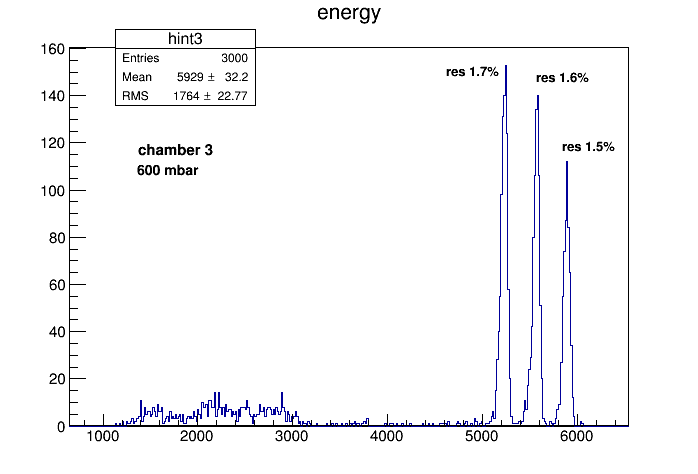
\includegraphics{../grafici/risultati/misura600_energy.png}
 }%
 \caption{Risoluzioni energetiche, grafico Energia(keV):conteggio} 
 \label{gr:600_energy.tex} 
\end{grafico}

\FloatBarrier
